\begin{frame}{Wariant angielski}

	% \hspace{1cm}

	% \begin{definicja}[Ezoteryczny język programowania]
	% 	Język zaprojektowany do badania niekonwencjonalnych technik programowania.
	% 	Taki język nie jest przeznaczony do pisania praktycznych aplikacji, mimo to jest \textbf{zupełny w sensie Turinga} (da się w nim zasymulować każdy możliwy program).
	% \end{definicja}

	Praca rozpatruje szczególną wersję Warcabów - \textbf{wariant angielski}.
	Wariant ten wprowadza dwie zmiany:
	\begin{itemize}
		\myitem Piony nie mogą poruszać się do tyłu,
		\myitem Damki nie ruszają się na dystansy większe niż jedno pole.
	\end{itemize}

	\begin{columns}
		\begin{column}{.5\hsize}
			{\centering
			\begin{figure}
				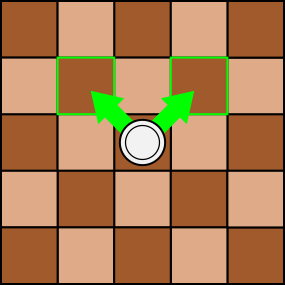
\includegraphics[scale=.25]{figures/warcaby_ruchyPionZwykle3.png}
				\caption{Ruchy dla piona}
			\end{figure}
			}
		\end{column}
		\begin{column}{.5\hsize}
			{\centering
			\begin{figure}
				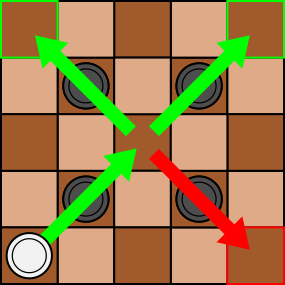
\includegraphics[scale=.25]{figures/warcaby_ruchyPionBicia.png}
				\caption{Bicia dla piona}
			\end{figure}
			}
		\end{column}
	\end{columns}

	\begin{columns}
		\begin{column}{.5\hsize}
			{\centering
			\begin{figure}
				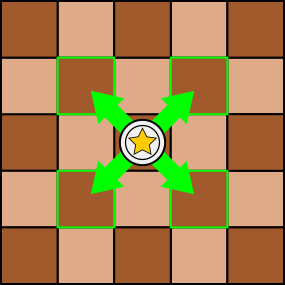
\includegraphics[scale=.25]{figures/warcaby_ruchyDamkaZwykle.png}
				\caption{Ruchy dla damki}
			\end{figure}
			}
		\end{column}
		\begin{column}{.5\hsize}
			{\centering
			\begin{figure}
				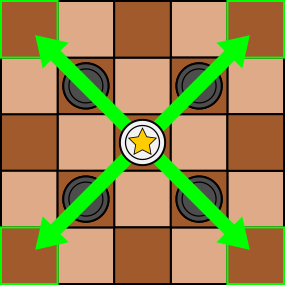
\includegraphics[scale=.25]{figures/warcaby_ruchyDamkaBicia.png}
				\caption{Bicia dla damki}
			\end{figure}
			}
		\end{column}
	\end{columns}

	% \begin{figure}
	% 	\centering
	% 	\begin{subfigure}{.5\textwidth}
	% 	  \centering
	% 	  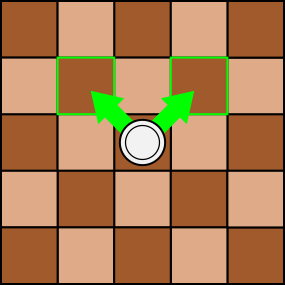
\includegraphics[scale=.6]{figures/warcaby_ruchyPionZwykle3.png}
	% 	  \caption{Legalne ruchy}
	% 	\end{subfigure}%
	% 	\begin{subfigure}{.5\textwidth}
	% 	  \centering
	% 	  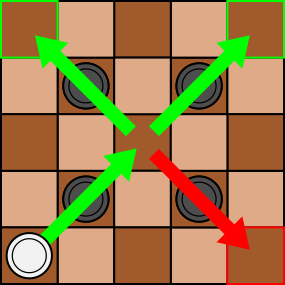
\includegraphics[scale=.6]{figures/warcaby_ruchyPionBicia.png}
	% 	  \caption{Legalne bicia}
	% 	\end{subfigure}
	% 	\caption{Zestaw możliwych ruchów dla piona w wariancie angielskim}
	% \end{figure}
		
	% \begin{figure}
	% 	\centering
	% 	\begin{subfigure}{.5\textwidth}
	% 	  \centering
	% 	  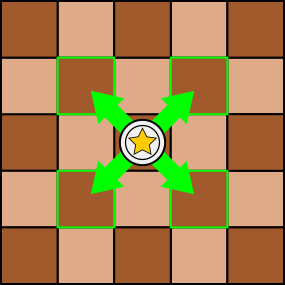
\includegraphics[scale=.6]{figures/warcaby_ruchyDamkaZwykle.png}
	% 	  \caption{Legalne ruchy}
	% 	\end{subfigure}%
	% 	\begin{subfigure}{.5\textwidth}
	% 	  \centering
	% 	  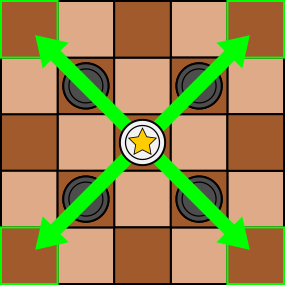
\includegraphics[scale=.6]{figures/warcaby_ruchyDamkaBicia.png}
	% 	  \caption{Legalne bicia}
	% 	\end{subfigure}
	% 	\caption{Zestaw możliwych ruchów dla damki w wariancie angielskim}
	% \end{figure}

	% \vspace{0.6cm}
	% {\hspace{7cm}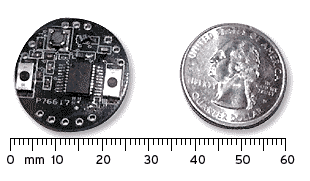
\includegraphics[height=2cm]{figures/mica2.png}}

\end{frame}
